% ============================================================================
%  SECCIÓN 6.3: MODELO DE DATOS EN POSTGRESQL
% ============================================================================

\section{Modelo de datos en PostgreSQL}

Antes de conectar la aplicaci\'on con Supabase se defini\'o la estructura
de datos que la aplicaci\'on necesita almacenar. El modelo responde a las
funcionalidades del proyecto definidas desde el inicio: escenarios
deportivos, deportes, eventos, favoritos, perfiles de usuario e
im\'agenes.

\subsection{Informaci\'on que almacena la aplicaci\'on}

A partir del an\'alisis del MVP se identificaron los datos que requieren
persistencia centralizada:

\begin{itemize}
  \item \textbf{usuarios:} perfiles con su rol de acceso (admin, gestor,
    asistente).
  \item \textbf{escenarios:} cat\'alogo de escenarios deportivos con su
    ubicaci\'on, capacidad y estado.
  \item \textbf{deportes:} disciplinas que se practican en cada escenario.
  \item \textbf{eventos:} actividades programadas en cada escenario.
  \item \textbf{favoritos:} escenarios guardados por cada usuario.
  \item \textbf{im\'agenes:} fotograf\'ias asociadas a cada escenario.
\end{itemize}

No se crean tablas sin relaci\'on con la aplicaci\'on: la estructura
responde a las funcionalidades previamente definidas.

\subsection{Entidades principales}

Cada entidad se convierte en una tabla de PostgreSQL:

\begin{enumerate}
  \item \textbf{profiles} (usuario).
  \item \textbf{scenarios} (escenario deportivo).
  \item \textbf{sports} (deporte).
  \item \textbf{scenario\_sports} (relaci\'on escenario--deporte).
  \item \textbf{events} (evento).
  \item \textbf{favorites} (favorito).
  \item \textbf{scenario\_images} (imagen del escenario).
\end{enumerate}

\subsection{Dise\~no de las tablas}

La correspondencia entre entidades y tablas se resume en la siguiente
tabla:

\begin{table}[H]
  \centering
  \caption{Entidades y tablas de la base de datos}
  \contenidoConFuente{%
    \begin{tablaAPA}
      \begin{tabular}{@{}p{3.2cm}p{3.4cm}p{7.0cm}@{}}
        \toprule
        \textbf{Entidad} & \textbf{Tabla} & \textbf{Prop\'osito} \\
        \midrule
        Usuario & profiles & Perfil del usuario y rol de acceso. \\
        \addlinespace
        Escenario deportivo & scenarios & Cat\'alogo de escenarios con
        ubicaci\'on y capacidad. \\
        \addlinespace
        Deporte & sports & Disciplinas disponibles. \\
        \addlinespace
        Escenario--deporte & scenario\_sports & Relaci\'on muchos a
        muchos entre escenarios y deportes. \\
        \addlinespace
        Evento & events & Actividades en cada escenario. \\
        \addlinespace
        Favorito & favorites & Escenarios guardados por el usuario. \\
        \addlinespace
        Imagen & scenario\_images & Fotograf\'ias de cada escenario. \\
        \bottomrule
      \end{tabular}
    \end{tablaAPA}%
  }{Elaboraci\'on propia en base al esquema de migraciones.}
\end{table}

\subsection{Definici\'on de campos}

Los campos de la entidad principal (escenario) responden a las necesidades
reales del proyecto:

\begin{table}[H]
  \centering
  \caption{Campos de la tabla \textit{scenarios}}
  \contenidoConFuente{%
    \begin{tablaAPA}
      \begin{tabular}{@{}p{3.2cm}p{3.6cm}p{6.4cm}@{}}
        \toprule
        \textbf{Campo} & \textbf{Tipo} & \textbf{Descripci\'on} \\
        \midrule
        id & uuid & Identificador \'unico (clave primaria). \\
        \addlinespace
        nombre & text & Nombre del escenario. \\
        \addlinespace
        tipo & text & Tipo: estadio, coliseo, cancha, etc. \\
        \addlinespace
        capacidad & integer & N\'umero de personas. \\
        \addlinespace
        direccion & text & Direcci\'on f\'isica. \\
        \addlinespace
        latitud, longitud & double precision &
        Coordenadas para el mapa. \\
        \addlinespace
        estado & text & activo o inactivo (soft delete). \\
        \addlinespace
        created\_by & uuid & Usuario que lo cre\'o (clave for\'anea). \\
        \bottomrule
      \end{tabular}
    \end{tablaAPA}%
  }{Elaboraci\'on propia en base a la migraci\'on 002.}
\end{table}

\subsection{Claves primarias y relaciones}

Cada tabla cuenta con una clave primaria que identifica de manera \'unica
cada registro, y las relaciones se establecen mediante claves for\'aneas:

\begin{table}[H]
  \centering
  \caption{Claves primarias y for\'aneas por tabla}
  \contenidoConFuente{%
    \begin{tablaAPA}
      \begin{tabular}{@{}p{3.0cm}p{4.4cm}p{6.0cm}@{}}
        \toprule
        \textbf{Tabla} & \textbf{Clave primaria} & \textbf{Claves for\'aneas} \\
        \midrule
        profiles & id & id $\rightarrow$ auth.users.id \\
        \addlinespace
        scenarios & id & created\_by $\rightarrow$ profiles.id \\
        \addlinespace
        events & id & scenario\_id $\rightarrow$ scenarios.id \\
        \addlinespace
        favorites & user\_id + scenario\_id &
        user\_id $\rightarrow$ profiles.id; scenario\_id
        $\rightarrow$ scenarios.id \\
        \addlinespace
        scenario\_sports & scenario\_id + sport\_id &
        scenario\_id $\rightarrow$ scenarios.id;
        sport\_id $\rightarrow$ sports.id \\
        \addlinespace
        scenario\_images & id & scenario\_id $\rightarrow$ scenarios.id \\
        \bottomrule
      \end{tabular}
    \end{tablaAPA}%
  }{Elaboraci\'on propia en base al esquema de migraciones.}
\end{table}

Las relaciones principales son: un usuario puede crear varios escenarios
(1:N), un escenario puede tener varios eventos (1:N), un usuario puede
guardar varios favoritos (1:N), y un escenario se relaciona con varios
deportes (N:N a trav\'es de \texttt{scenario\_sports}). El diagrama
entidad--relaci\'on se presenta a continuaci\'on:

\begin{figure}[H]
\centering
  \figuraAPA{fig:diagrama-er-supabase}{Diagrama entidad--relaci\'on del modelo de datos}{%
  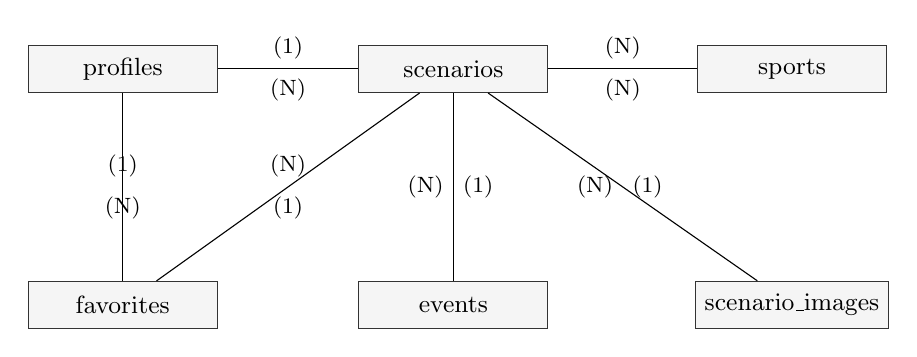
\begin{tikzpicture}[
    entity/.style={rectangle, draw=black!80, fill=gray!8,
      minimum width=2.4cm, minimum height=0.6cm, align=center,
      font=\small},
    rel/.style={diamond, draw=black!60, fill=gray!5,
      minimum width=1.1cm, minimum height=0.5cm, align=center,
      font=\footnotesize},
    line/.style={-}
  ]
    % Entidades
    \node[entity] (profile) at (0, 3) {profiles};
    \node[entity] (scenario) at (4.2, 3) {scenarios};
    \node[entity] (sport) at (8.5, 3) {sports};
    \node[entity] (event) at (4.2, 0) {events};
    \node[entity] (fav) at (0, 0) {favorites};
    \node[entity] (img) at (8.5, 0) {scenario\_images};

    % Relaciones
    \draw[line] (profile) -- node[above, font=\footnotesize]
      {(1)} node[below, font=\footnotesize] {(N)} (scenario);
    \draw[line] (scenario) -- node[above, font=\footnotesize]
      {(N)} node[below, font=\footnotesize] {(N)} (sport);
    \draw[line] (scenario) -- node[right, font=\footnotesize]
      {(1)} node[left, font=\footnotesize] {(N)} (event);
    \draw[line] (profile) -- node[above, font=\footnotesize]
      {(1)} node[below, font=\footnotesize] {(N)} (fav);
    \draw[line] (fav) -- node[above, font=\footnotesize]
      {(N)} node[below, font=\footnotesize] {(1)} (scenario);
    \draw[line] (scenario) -- node[right, font=\footnotesize]
      {(1)} node[left, font=\footnotesize] {(N)} (img);
  \end{tikzpicture}
  }{Elaboraci\'on propia.}
\end{figure}

\subsection{Creaci\'on de las tablas con SQL}

Las tablas se crearon mediante archivos de migraci\'on de Supabase. El
siguiente extracto corresponde a la creaci\'on de la tabla de escenarios
y de eventos:

\begin{lstlisting}
CREATE TABLE public.scenarios (
  id UUID PRIMARY KEY DEFAULT gen_random_uuid(),
  nombre TEXT NOT NULL,
  tipo TEXT NOT NULL,
  descripcion TEXT NOT NULL DEFAULT '',
  capacidad INTEGER NOT NULL DEFAULT 0,
  direccion TEXT NOT NULL DEFAULT '',
  latitud DOUBLE PRECISION NOT NULL DEFAULT 0,
  longitud DOUBLE PRECISION NOT NULL DEFAULT 0,
  estado TEXT NOT NULL DEFAULT 'activo',
  created_by UUID REFERENCES public.profiles(id)
    ON DELETE SET NULL,
  created_at TIMESTAMPTZ NOT NULL DEFAULT NOW(),
  updated_at TIMESTAMPTZ NOT NULL DEFAULT NOW()
);

CREATE TABLE public.events (
  id UUID PRIMARY KEY DEFAULT gen_random_uuid(),
  scenario_id UUID NOT NULL
    REFERENCES public.scenarios(id) ON DELETE CASCADE,
  nombre TEXT NOT NULL,
  fecha DATE NOT NULL,
  hora TIME NOT NULL DEFAULT '00:00',
  descripcion TEXT NOT NULL DEFAULT '',
  created_at TIMESTAMPTZ NOT NULL DEFAULT NOW(),
  updated_at TIMESTAMPTZ NOT NULL DEFAULT NOW()
);
\end{lstlisting}

El concepto fundamental detr\'as del script es: \texttt{CREATE TABLE}
crea la tabla, \texttt{PRIMARY KEY} establece el identificador \'unico y
\texttt{REFERENCES} define la relaci\'on con otra tabla. La seguridad de
los datos se refuerza con pol\'iticas de seguridad a nivel de fila
(RLS) sobre cada tabla, de modo que cada usuario s\'olo accede a la
informaci\'on que le corresponde.